
\section{Introduction}
This guide is intended to help newcomers get started with segmentation tasks in a software called ``3D Slicer''.
3D Slicer is a comprehensive and fully featured program for visualization, processing, segmentation, registration and analysis of 3D datasets.
Unfortunately, this also means that it can be overwhelming for someone who lacks experience working with such tools.
This guide aims to alleviate this issue at least for segmentation workflows.
It tries to explain tools and possible workflows in an easy-to-follow manner and enable the reader to complete their segmentation without needing to watch multiple tutorials or read bits of documentation scattered around the internet.

\subsection{Using the guide}
\begin{description}
	\item [1. Jump around using links:] The guide makes extensive use of hyperlinks, which enable the reader to easily jump to important information. Make use of this feature to save yourself some time. Note that most but not all PDF readers will support this feature.
	\item [2. Jump to information you require:] This guide covers many tools and functionalities of 3D Slicer. You will most certainly not use every tool. Use the table of contents to jump to tools that are important for the task at hand.
	\item [3. Make a backup before experimenting:] Sometimes 3D Slicer makes it difficult to undo an operation. If you wish to experiment with a tool you have never used before it is advisable to duplicate your dataset and save it to a separate file. So that in case something does not turn out the way you intended, and you do not know how to undo the unwanted change, you can always load a known good copy of your dataset.
\end{description}

\subsection{Conventions used in this Guide}

\begin{figure}[h]
	\begin{centering}
		\begin{subfigure}{0.5\textwidth}
			\includesvg[
				inkscapelatex=false,
				width = 0.6\linewidth
			]{2d.svg}
			\caption{2D symbol}
			\label{fig:2d_icon}
		\end{subfigure}
		\begin{subfigure}{0.5\textwidth}
			\includesvg[
				inkscapelatex=false,
				width = 0.6\linewidth
			]{3d.svg}
			\caption{3D symbol}
			\label{fig:3d_icon}
		\end{subfigure}
	\end{centering}
	\caption{2D (\cref{fig:2d_icon}) and 3D (\cref{fig:3d_icon}) symbols signifying if a tool can be used in 2D or 3D}
\end{figure}

\begin{figure}[h]
	\begin{centering}
		\begin{subfigure}{0.5\textwidth}
			\includesvg[
				inkscapelatex=false,
				width = 0.6\linewidth
			]{hint.svg}
			\caption{Hint symbol}
			\label{fig:hint_icon}
		\end{subfigure}
		\begin{subfigure}{0.5\textwidth}
			\includesvg[
				inkscapelatex=false,
				width = 0.6\linewidth
			]{irreversible.svg}
			\caption{Irreversible symbol}
			\label{fig:noundo_icon}
		\end{subfigure}
	\end{centering}
	\caption{Hint (\cref{fig:hint_icon}) symbol signifying tip or hint and Irreversible(\cref{fig:noundo_icon}) symbol signifying irreversible operation}
\end{figure}

\begin{figure}[h]
	\begin{centering}
		\begin{subfigure}{0.5\textwidth}
			\includesvg[
				inkscapelatex=false,
				width = 0.6\linewidth
			]{performance.svg}
			\caption{Performance symbol}
			\label{fig:performance_icon}
		\end{subfigure}
		\begin{subfigure}{0.5\textwidth}
			\includesvg[
				inkscapelatex=false,
				width = 0.6\linewidth
			]{plugin.svg}
			\caption{Plugin symbol}
			\label{fig:plugin_icon}
		\end{subfigure}
	\end{centering}
	\caption{Performance(\cref{fig:performance_icon}) symbol signifying resource intensive operation and Plugin (\cref{fig:plugin_icon}) symbol signifying 3rd party plugin tool}
\end{figure}


\noindent
If you are already familiar with 3D Slicer and want to start with the segmentation right away, skip to page \pageref{section:quickstart} for the Quick Start Guide.

\subsection{Installation}
Basic installation instructions for 3D Slicer:
\begin{enumerate}
	\item Browse to: \url{https://download.slicer.org}
	\item Download the installer of the latest stable release\footnote{Version 5.6.2 at the time of writing this document} for your operating system
	\item Run the installer and follow its instructions
\end{enumerate}

\subsubsection{Installation on macOS}
On macOS, 3D Slicer can be installed in two different ways:\newline\newline
Either via the provided package on the downloads page, or via Homebrew: \url{https://formulae.brew.sh/cask/slicer}\newline
For the conventional installation refer to the 3D Slicer wiki: \url{https://slicer.readthedocs.io/en/latest/user_guide/getting_started.html#mac}

\subsubsection{Installation on Linux}
3D Slicer ships with all its dependencies on Windows and macOS.\\
On Linux it is required to install some dependencies via your distributions package manager.\\
The 3D Slicer wiki gives information about required packages and their respective names on different distributions:
\url{https://slicer.readthedocs.io/en/latest/user_guide/getting_started.html#linux}.\\
To make this process easier, this guide provides a distrobox manifest file (see page: \pageref{code:distrobox-manifest}), which allows the user to create a Linux container holding all necessary dependencies without polluting the host system.\newline\newline
To run 3D Slicer via the container run:
\inputminted[
	%fontsize=\footnotesize, % set text size
	stripnl, % strip leading newlines
	numbers=left, % display line numbers on the left
	breaklines % break lines after spaces if necessary
]{sh}{./code/runSlicer.sh}

\subsection{System Requirements\cite{fedorov3DSlicerImage2012}}
Note: as of \today
\subsubsection{Official supported operating systems}
\begin{itemize}
	\item Windows: 10 or 11
	\item macOS: 11 or later
	\item Linux:
	      \begin{itemize}
		      \item Ubuntu 20.04 or later
		      \item Debian 10 or later
		      \item Fedora 35 or later
		      \item CentOS 7 or later
	      \end{itemize}
\end{itemize}

\subsubsection{Hardware requirements}
\begin{itemize}
	\item Memory: At least 4 Gigabytes, more is strongly recommended.\\The 3D Slicer Wiki mentions needing about 10 times more memory than the amount of data you plan to load.\\ 3D Slicer on its own uses about 456 Megabytes of RAM. After loading a 26.17MiB Dataset it consumes about 614 MB.
	\item \gls{cpu}: 3D Slicer uses multi-threading for some calculation and will thus benefit from a multicore CPU.
	\item \gls{gpu}: A dedicated GPU is recommended but not required as 3D Slicer only uses it for interactive volume rendering. If you restrict your usage to the 2D views, you will hardly ever use your graphics card.
\end{itemize}

\subsubsection{Hardware recommendations}
The following points are not strictly needed in order to use 3D Slicer, but they make working with the software a lot easier.
\begin{itemize}
	\item Input devices: 3D Slicer supports mice, touchpads, pens, graphic tablets and \gls{openvr} headsets. The easiest input method though is a 3 button Mouse with a mouse wheel.
	\item Internet connection: for downloading extensions, online documentation and sample data sets.
	\item \gls{vram}: for interactive volume rendering it is recommended to have more GPU texture memory than the data set you plan to load.
	\item A large display or monitor with a decent screen resolution. A 14-inch screen or larger is strongly advised. Screen resolution does not need to exceed 1920x1080, but going below 720p is also not advisable.
\end{itemize}


\subsection{Interface and Usage}
Upon first launch you will be greeted by the 3D Slicers welcome screen (\cref{fig:slicerWelcome})
\begin{figure}[h!] % h - here
	\centerline{
		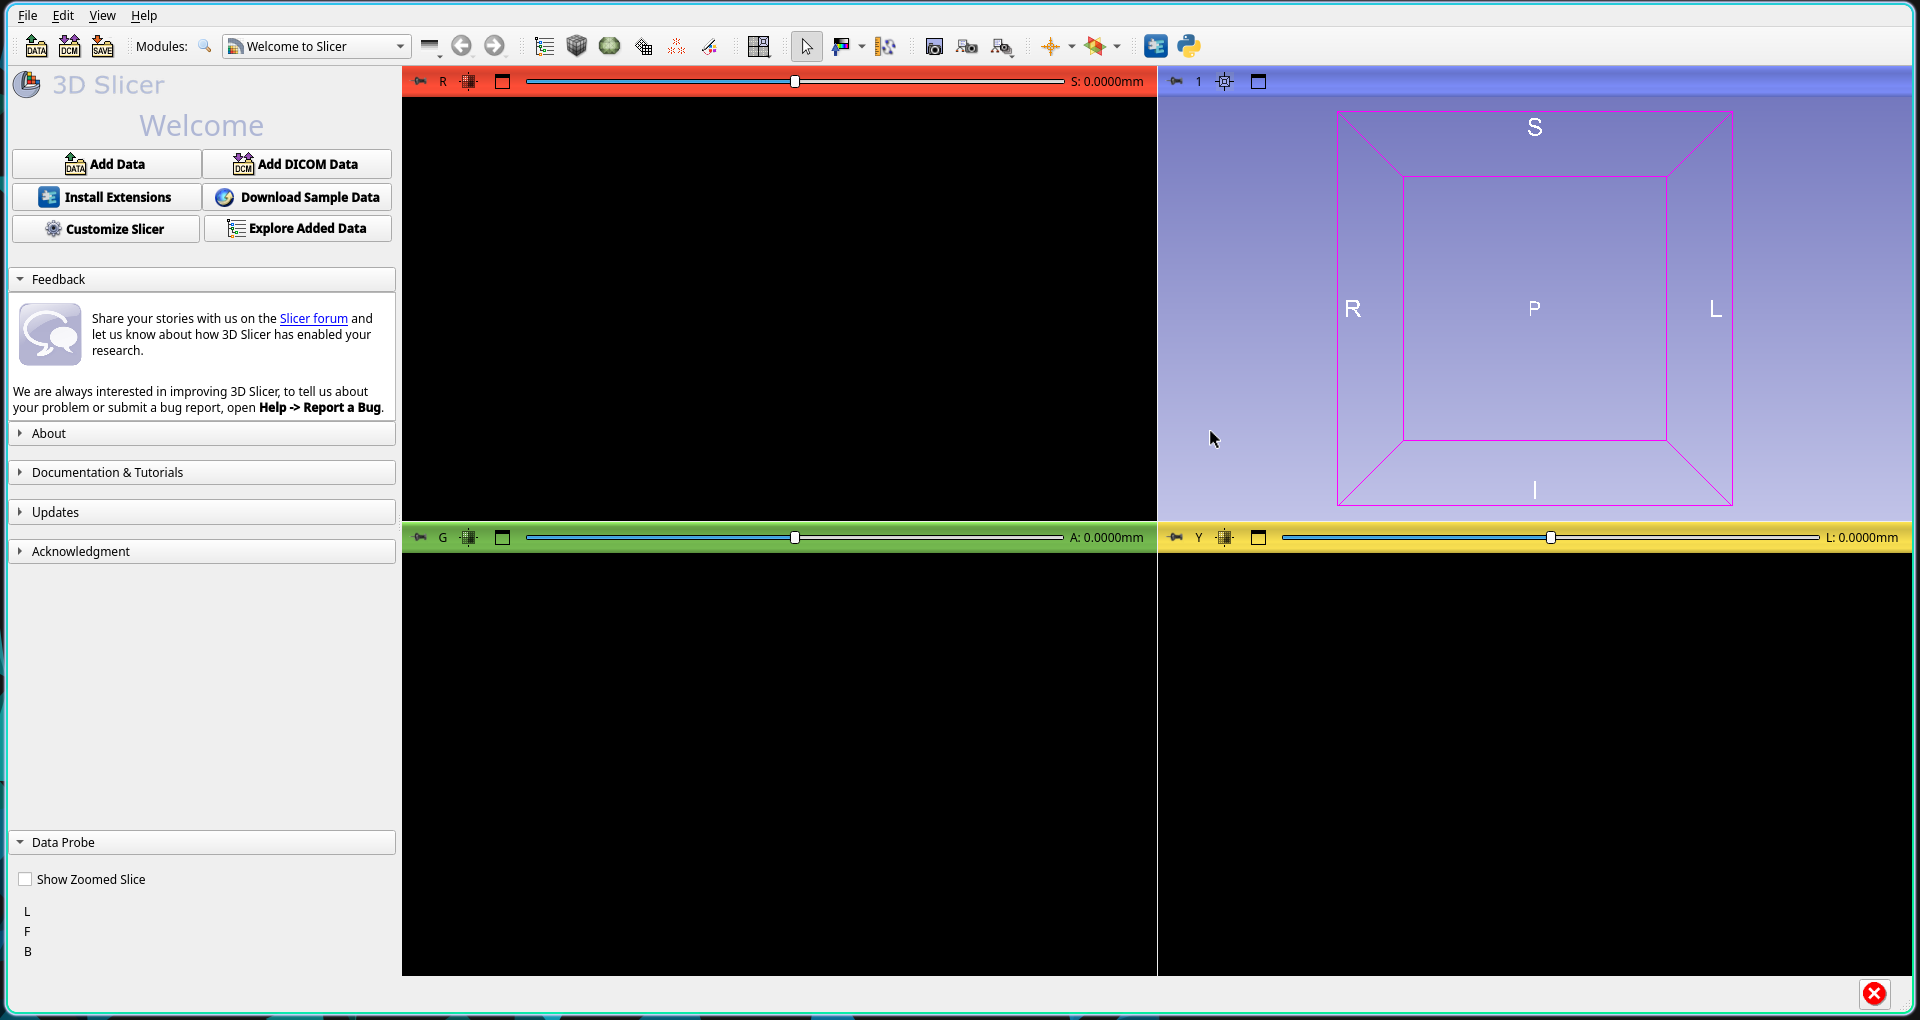
\includegraphics[
			% scale=0.2
			width=1.1\textwidth
		]{slicerWelcome.png}}
	\caption{3D Slicer welcome screen}\label{fig:slicerWelcome}
\end{figure}
\noindent
The welcome screen has some quick links to useful modules like load data and download datasets.
\pagebreak
\begin{figure}[h!] % h - here
	\centerline{ % center a single element on page, from: https://tex.stackexchange.com/a/4438
		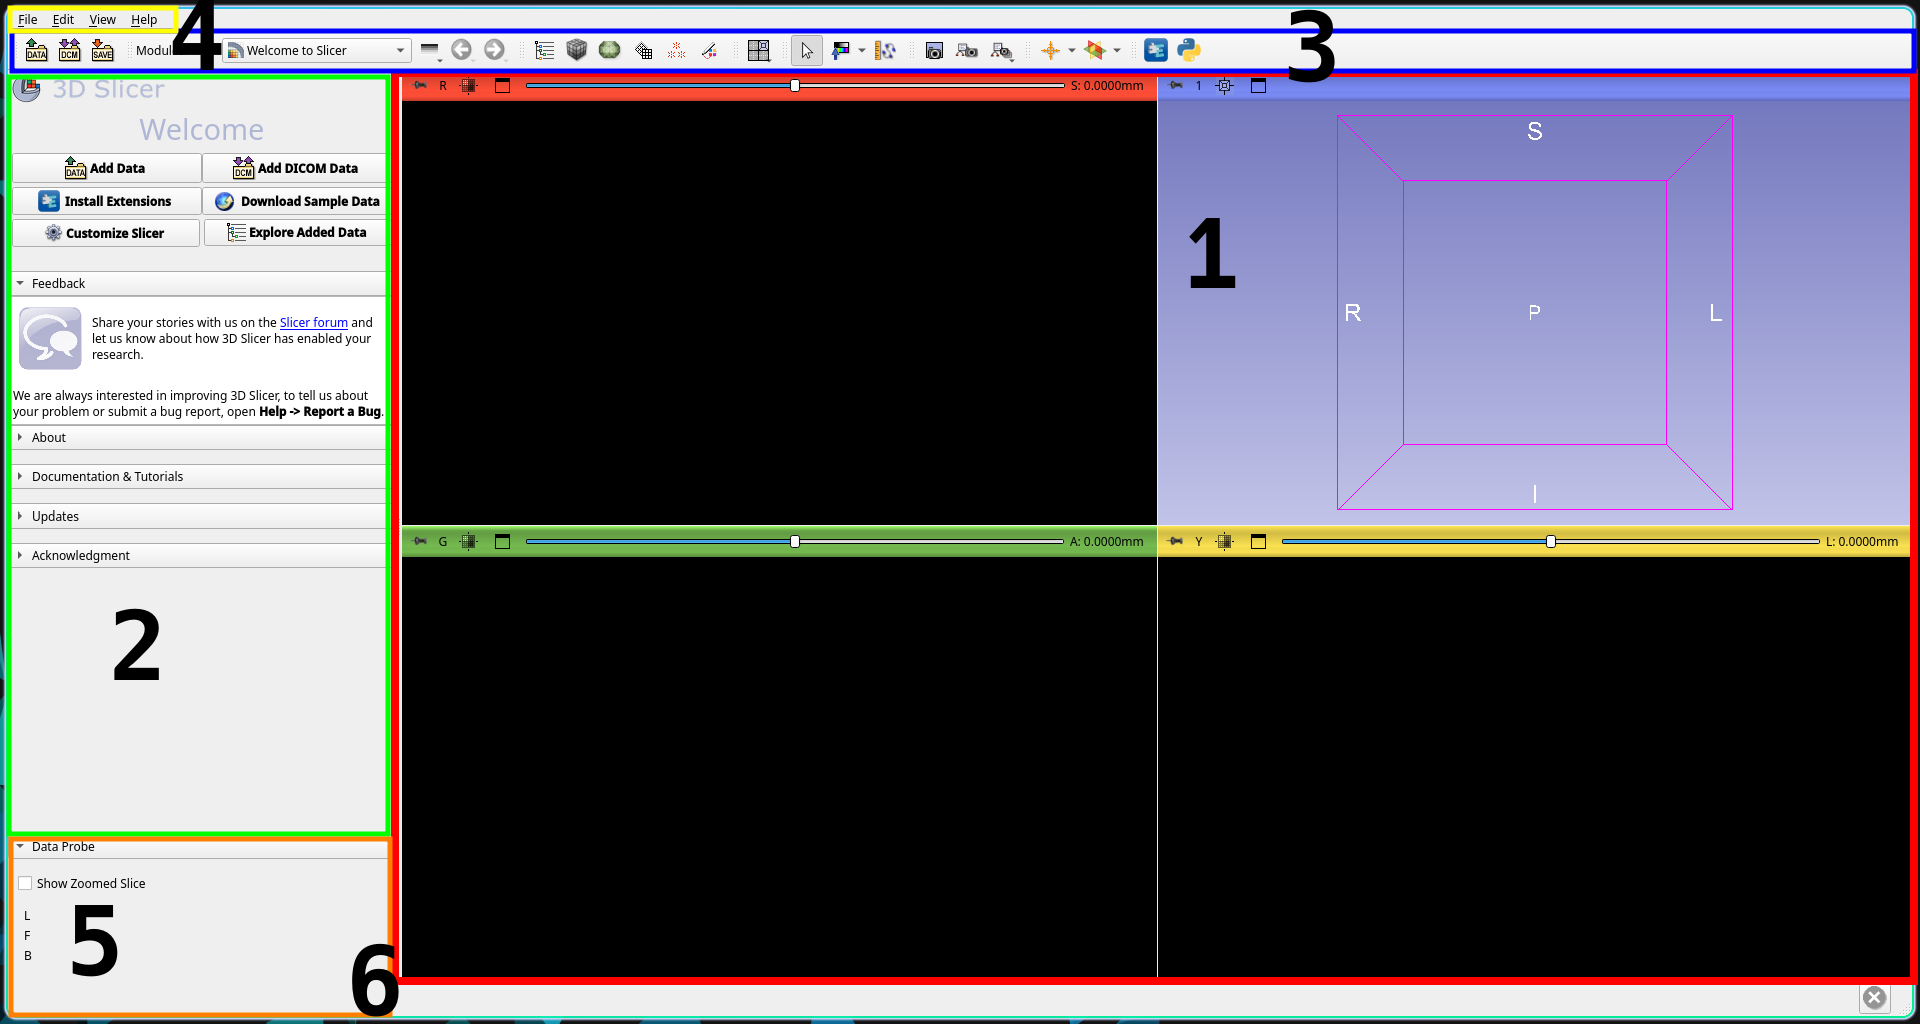
\includegraphics[
			% scale=0.2
			width=1.1\textwidth
		]{slicerWelcomeMarked1.png}}
	\caption{3D Slicer window}\label{fig:slicerView}
\end{figure}

\noindent
The 3D Slicer window consists of several areas, which provide different tools to interact with the program.
A quick overview of these areas is provided by \cref{fig:slicerView}:
\begin{enumerate}
	\item View area
	\item Module panel
	\item Toolbar
	\item Application menu
	\item Data probe
	\item Status bar
\end{enumerate}

\pagebreak

\subsubsection{The view area}\label{sec:view_area}
By default 3D Slicer shows the view area (\cref{fig:4upview}) with three 2D slice views and the interactive 3D view at the top right.\\
\noindent
\begin{figure}[h!] % h - here
	\centerline{ % center a single element on page, from: https://tex.stackexchange.com/a/4438
		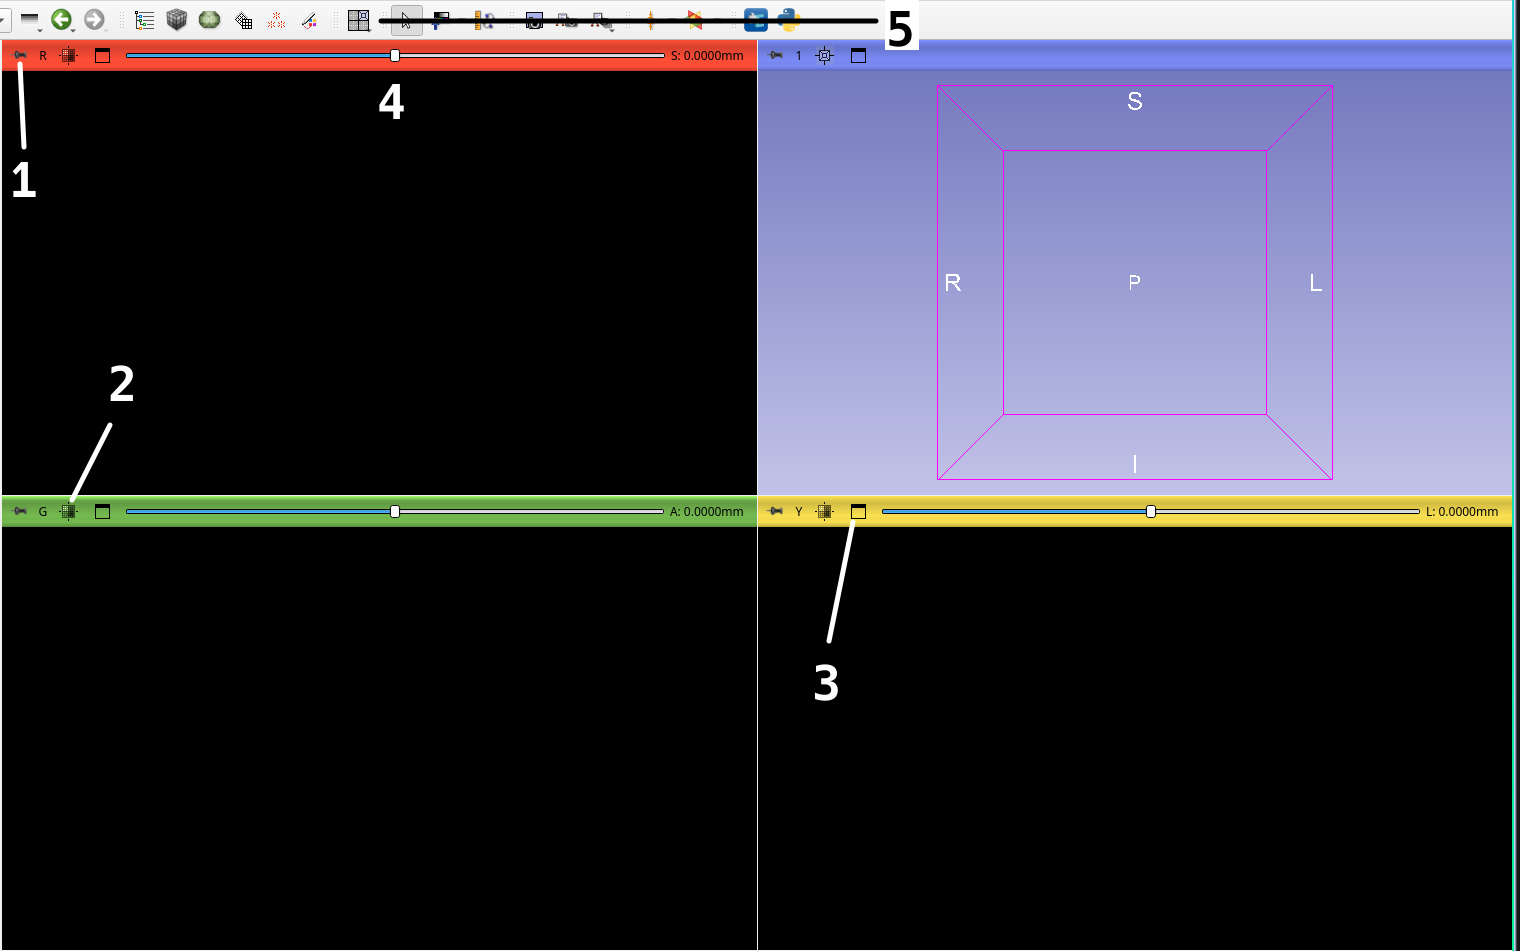
\includegraphics[
			% scale=0.2
			width=1.1\textwidth
		]{view.png}}
	\caption{3D Slicer view area}\label{fig:4upview}
\end{figure}

\noindent
3D Slicer calls this the \texttt{Four-up} view.\\

\noindent
There is a numerous amount of view presets to choose from by clicking on the \texttt{change view} option in the toolbar: \cref{fig:4upview}:5.\\

\noindent
Each slice view has its own scroll bar (\cref{fig:4upview}:4).
The number on the right end of the scroll bar shows by how much a single tick scrolls through the dataset.
In other words: it shows the slice thickness of the view.\\
\noindent
Scrollbar controls:
\begin{itemize}
	\item left click and drag the scrollbar
	\item mouse wheel
	\item \texttt{B} and \texttt{F} Keys
	\item up, down, left and right arrow keys
\end{itemize}

\noindent
To maximize a single slice view, click on the \texttt{Maximize view} button (\cref{fig:4upview}:3). Click it again to return to the previous layout. Double left-clicking on the slice has the same effect.\\

\noindent
'Reset \gls{fov}' can be used to reset the zoom level and shift the slice into its isocenter (\cref{fig:4upview}:2). The \texttt{R} key has the same effect.\\

\noindent
The pin icon (\cref{fig:pinMenu}:1) brings up a submenu.\\
\noindent
Here (\cref{fig:pinMenu}:2) it is possible to quickly change the displayed dataset if more than one has been loaded.\\
Change the displayed slice plane by clicking on \cref{fig:pinMenu}:3.\\
Toggle slice visibility in 3D views: \cref{fig:pinMenu}:4.\\
Clicking on the \texttt{double arrow} button (\cref{fig:pinMenu}:5) will reveal more configuration options, which this guide will not cover, as they are not usually needed for segmentation tasks.
However, the 3D Slicer documentation provides more information about this submenu: \url{https://slicer.readthedocs.io/en/latest/user_guide/user_interface.html#slice-view}
\begin{figure}[h!] % h - here
	\centerline{ % center a single element on page, from: https://tex.stackexchange.com/a/4438
		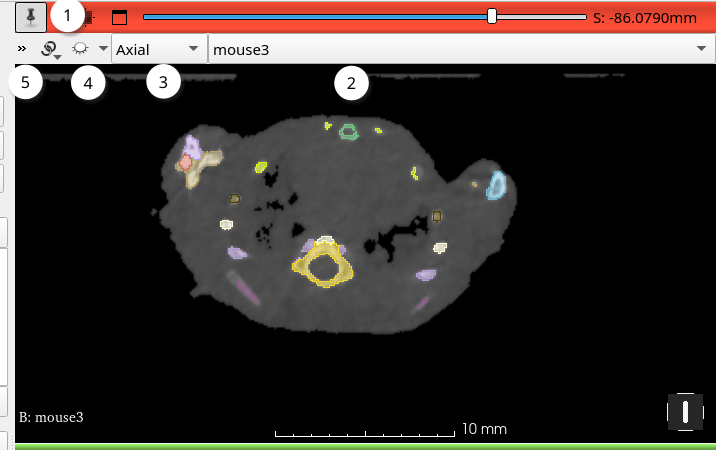
\includegraphics[
			% scale=0.2
			width=1.1\textwidth
		]{pinMenu.png}}
	\caption{3D Slicer pin menu}\label{fig:pinMenu}
\end{figure}
\pagebreak

\subsubsection{The module panel}
\Cref{fig:slicerView}:2 the module panel displays options, tools and information of the currently loaded module.

\subsubsection{The Toolbar}
\begin{figure}[h!] % h - here
	\centerline{ % center a single element on page, from: https://tex.stackexchange.com/a/4438
		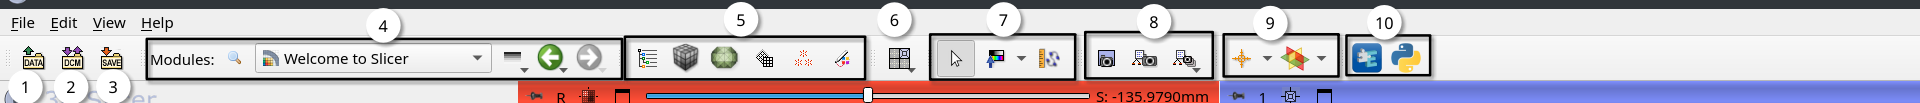
\includegraphics[
			% scale=0.2
			width=1.2\textwidth
		]{toolbar.png}}
	\caption{3D Slicer toolbar}\label{fig:toolbar}
\end{figure}

\noindent
The far left end of 3D Slicers toolbar holds buttons for loading and saving data.
Loading data from a file or directory can be done via the \texttt{Add Data} button' \cref{fig:toolbar}:1.\\
Keyboard shortcut: \texttt{Ctrl + o}\\
The next button (\cref{fig:toolbar}:2) loads the \texttt{Add DICOM Data} module, which can also load data from files or directories and save it to 3D Slicers on disk DICOM database.\\
Saving data can be done via clicking on the \texttt{Save Data} button (\cref{fig:toolbar}:3).\\Keyboard shortcut: \texttt{Ctrl + s}\\
\Cref{fig:toolbar}:4 marks the module toolbar. Clicking on the lens button opens a full text search for all installed modules.\\
Keyboard shortcut: \texttt{Ctrl + f}\\
Loadable modules can also be found via the dropdown list right next to the lens icon.
3D Slicer keeps track of the recently used modules and allows to quickly return to the most recent eight\footnote{the amount can be configured in the settings menu} modules.
Either via the \texttt{Modules history} dropdown list or the forward and back buttons (\cref{fig:toolbar}:4).
The toolbar has a designated part for \texttt{Favorite Modules} (\cref{fig:toolbar}:5), which can be fully customized via the settings menu.\\
\Cref{fig:toolbar}:6 can be used to change the view layout, like mentioned in \cref{sec:view_area}.\\
3D Slicer has different mouse modes, where depending on the selected mode, the mouse has different functionalities. By default, \texttt{translate/rotate view} is selected (\cref{fig:toolbar}:7).\\
Keyboard shortcuts:\\
\texttt{right click + mouse drag} to zoom in and out.\\
\texttt{Ctrl + mouse wheel} to zoom in and out.\\
\texttt{Shift + left mouse click + drag} pan view.\\
\texttt{Shift + move mouse} display ROI under mouse in all views, 3D Slicer calls this the crosshair.\\
\noindent
The icon to the right is called \texttt{adjust window/level}.\\
\texttt{Left click} and drag to create a ROI, 3D Slicer then tries to find the optimal window and center for that ROI.\\
Alternatively hold \texttt{Ctrl} and \texttt{left mouse}, then drag the mouse to adjust the window manually.\\
The final button of this part of the toolbar toggles an additional markups toolbar on and off, this guide will not go into further detail as this is not needed for segmentation.\\
3D Slicer has a build in screenshot and screen recording module as can be seen in \cref{fig:toolbar}:8.\\
To toggle visibility of the crosshair, that has been mentioned above the left button in \cref{fig:toolbar}:9 can be used. The button to the right of that toggles slice intersection lines on and off.\\
Finally, on the right end (\cref{fig:toolbar}:10) of the toolbar 3D Slicer has buttons to open a Python console window and opening the \texttt{Extension Manager}.

\subsubsection{The Application Menu}
See \cref{fig:slicerView}:4.
\begin{itemize}
	\item \texttt{File}: Loading and saving data, download sample data, unloading data and close 3D Slicer
	\item \texttt{Edit}: Cut, Copy, Paste and the \texttt{Settings Menu}
	\item \texttt{View}: Show or hide additional windows and toolbars. Open the \texttt{Extension Manager}, \texttt{Python console}, \texttt{Error Log} and change the view layout.
	\item \texttt{Help}: Access online documentation.
\end{itemize}

\subsubsection{The Data Probe}
\begin{figure}[h!] % h - here
	\centerline{ % center a single element on page, from: https://tex.stackexchange.com/a/4438
		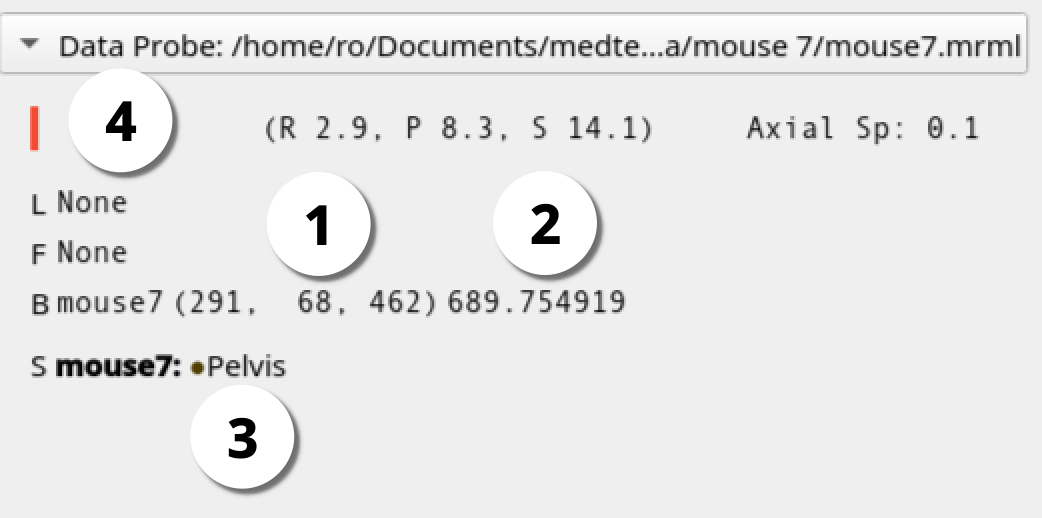
\includegraphics[
			% scale=0.2
			width=1.1\textwidth
		]{dataprobe.png}}
	\caption{3D Slicer Dataprobe}\label{fig:dataprobe}
\end{figure}

\noindent
The \texttt{Data Probe} shows useful information about the data currently being displayed. More specifically it informs the user about the ROI under the cursor position.\\
To start using it, just hover the mouse cursor over a ROI, if the cursor is moved, the data probe will update in real time.\\
Most notable information shown:\\
The numbers in brackets in \cref{fig:dataprobe}:1 display the x-, y- and z-Position of the ROI. After that, outside the brackets, it displays the \gls{hu} value of that ROI (\cref{fig:dataprobe}:2).\\
In \cref{fig:dataprobe}:3 the data probe shows which segmentation ROI belongs to if any.\\
\Cref{fig:dataprobe}:4 displays the currently loaded dataset.

\subsubsection{The Status Bar}
The status bar located on the bottom of the 3D Slicer window, is of no great importance during normal operation. Notably the \texttt{X} icon on the far right opens the error log, which may be useful for debugging.

% \pagebreak
% Für das Arbeiten mit Quellen, empfehle ich Zotero (oder Mendeley).
% Natürlich geht's auch die Quellen direkt aus zB Scholar im \textit{bibtex} Format ins Verzeichnis (= *.bib-Datei) zu kopieren.

% \subsubsection{Auf Grafiken kann selten verzichtet werden}
% Grafiken

% \subsubsection{Formeln sind in der angewandeten Informatik seltener anzutreffen}
% Die folgende Formel ist als eigenständige Formel nummeriert:
% \begin{equation}
% 	\frac{\partial^2 }{\partial x^2}  % Online Formeleditor (google!) wirkt Wunder!
% \end{equation}

% Formeln können aber auch direkt in den Text $\frac{\partial^2 }{\partial x^2}$, was allerdings schwer zu lesen ist.
% Für die Formeln in \LaTeX gibt's im Web eigene \textit{Cheat Sheets}, schließlich wurde es extra für den Formelsatz entwickelt.


% \subsubsection{Tabellen gehören ohne Gitternetzlininen (booktabs Stil)}
% Tabellen im Booktabs Stil sind professioneller gestaltet und lenken nicht durch Gitternetzlinien ab. Das ist gut so, denn welche Daten haben es schon verdient, ihr Leben hinter Gittern zu verbringen?
% Zum Glück, gibt's dafür Online Editoren, denn von der Usability her, ist das händische Setzen einer Tabelle eine Katastrophe.

% % \begin{table}[h]

% % \centering
% % \begin{tabular}
% %\toprule
% % ID & \multicolumn{1}{l}{Farbe} & \multicolumn{1}{l}{Anteil} \\ \midrule
% % 1  & rot                       & 255                        \\
% % 2  & grün                      & 255                        \\
% % 3  & blau                      & 0                          \\ \bottomrule
% % \end{tabular}
% % \caption{Tabellen werden fallweise auch oben beschriftet. Dann einfach die caption im Quellcode an die richtige Stelle verschieben.}
% % \end{table}


% \subsubsection{Programmcode darf nur auszugsweise in die Arbeit}

% Eigentlich gehören komplette Codelistings in den Anhang.
% Wenn aber in der Arbeit zB ein Algorithmus erläutert werden soll, dann gehört das natürlich direkt in die Arbeit.

% Verbatim ist dabei die einfachste Variante für Programmcode.
% Ausgefeilter geht's dann zB mit lstlistings zur Sache, wo auch Syntax Highlighting vorgenommen werden kann. \\

% Müssen Klassen-/Methoden-/Variablennamen im Fließtext erwähnt werden, bietet sich ein Inline-Verb-Block an, mit dem kann auf eine \verb|Class1.Method1()| Bezug genommen werden, ohne dass diese als zu lesendes Wort missverstanden wird. %PHR

% \subsubsection{Wie man mit Aufzählungen verfährt}

% Nummerierte Aufzählungen werden nur dann eingesetzt, wenn wirklich eine Reihenfolge vorliegt.
% Kann auch geschachtelt werden (siehe Beispiel).

% \begin{enumerate}
% 	\item Erster Schritt
% 	\item Zweiter Schritt
% 	      \begin{enumerate}
% 		      \item erster Subschritt zu Schritt zwei
% 		      \item zweiter Subschritt zu Schritt zwei
% 	      \end{enumerate}
% 	\item Dritter Schritt
% \end{enumerate}

% Aufzählungen, die keine zwingende Reihenfolge wiedergeben werden durch \textit{Bullet Points} formatiert.
% In folgenden Beispiel wird auf Schachtelung verzichtet, obwohl sie ohne weiteres möglich wäre.

% \begin{itemize}
% 	\item grüner Tee
% 	\item schwarzer Tee
% 	\item weisser Tee
% 	\item aromatisierter Tee
% 	\item Kräuterteee
% \end{itemize}

% \subsubsection{Ein paar persönliche Tipps zum Arbeiten - bitte ohne Scheu ergänzen!}

% Jeden Satz in einer eigenene Zeile - das hab ich zwar schon erwähnt, ist für mich aber eine wirkliche Hilfe, wenn man sich einmal daran gewöhnt hat.

% Hervorhebungen im Text \textit{nie} mit fett oder unterstrichen, sonderm \textit{immer} mit kursivem Text.
% Das kriegt man entweder durch \textit{textit} hin oder \textit{emph}

% (Harte) Zeilenumbrüche macht man mit einem doppelten Backslash, Absatzumbrüche hingegen durch mehr als 2 Absatzschaltungen im Quelltext.
% Die Anzahl der Leerzeilen wird dabei nicht berücksichtigt, was zur schöneren Strukturierung des Quelltexts beiträgt.

% Kommentare helfen, nichts zu vergessen.
% % nicht vergessen!

% Quick \& Dirty -- die Rohversion der Arbeit sollte möglichst zügig verfasst werden.
% Das hilft, den roten Faden nicht zu verlieren.
% Überarbeiten, umformulieren, Grafiken usw einfügen und überhaupt verschönern kann man später.

% Warnungen (gelbes Dreieck) in Overleaf betreffen meist \textit{overfull boxes} d.h. der Text ist zu lang.
% Bis zur finalen Version können diese ignoriert werden.
% Fallen sie dann tatsächlich ins Gewicht (nur dann!) kann man versuchen, diese durch manuelle Silbentrennung hinzukriegen.

% Querverweise verwenden die \textit{labels} zB bei Grafiken oder Tabellen und werden mit \textit{ref} oder \textit{pageref} eingefügt.

% Fast nicht zu entdecken: die kleinen Dreiecke neben den Zeilennummern in Oveleaf.
% Damit kann man den Bereich \textit{einfalten}, was zur Übersicht beiträgt.

% Wenn man in der Vorschau doppelt in den Text klickt, springt man im Editor auf die Stelle im LaTeX-Quellcode.

% Wenn man länger AFK war, dann kann's sein, dass man aus Overleaf abgemeldet ist.
% Bei mir hat's noch NIE funktionert, sich über Button neu zu verbinden - es war immer ein Aussteigen - Einsteigen notwendig.

% Wer sich von den überwältigenden Möglichkeiten mit LaTeX beeindrucken lassen will, googelt nach \textit{Tikz}.
% Da gibt's dann fast Nix, was es nicht gibt.

% Grundsätzlich ist bei der Arbeit mit \LaTeX Google ein guter Freund.
% Die Community ist riesig und was man nicht in der sehr guten Hilfe von Overleaf findet, hat in den allermeisten Fällen jemand anderer schon gepostet.
